\documentclass[a4paper,12pt]{article}
\usepackage{polski}
\usepackage[utf8]{inputenc}
\usepackage[OT4]{fontenc}
\usepackage{mathtools}
\usepackage{float}
\usepackage{graphicx}
\usepackage{multirow}

\newcommand{\h}[1]{\noindent \bf #1 \rm \\ \noindent}
\newcommand{\italic}[1]{\it #1 \rm}

\begin{document}

\begin{center}
	\LARGE
	Architektura Komputerów 2 \\
	\large
	WYKŁAD 2 
\end{center}
\vspace{1cm}

\h{Rozkaz/instrukcja:}
Implementowana przez procesor instrukcja. Pojedynczy, niepodzielny składnik programu (niezależna jednostka syntaktyczna). Co ważne jedna instrukcja może składać się z wielu "pól taśmy" (wielu bajtów).\\

\h{Typy instrukcji w procesorach:}
Pierwszym typem instrukcji procesora są instrukcje wykonujące działania na danych (właściwe instrukcje procesora). Podstawowymi instrukcjami takiego typu są (wymienione rosnąco względem skomplikowania):
\begin{itemize}
	\item \italic{kopiowanie} - np. z pamięci do rejestru
	\item \italic{zmiana formatu} - rotacje, przesunięcia, proste przemieszczenia pól
	\item \italic{konwersje kodu} - np. z U2 na ZM poprzez dodawanie lub usuwanie bitów
	\item \italic{działania logiczne} - jednobitowe lub działające na bitach słów
	\item \italic{działania arytmetyczne} - dodawanie, odejmowanie, mnożenie itd.
\end{itemize}
\vspace{5mm}

\noindent
Drugim typem instrukcji są instrukcje sterujące zachowaniem i ruchem "głowicy" odczytującej pola z pamięci kodowej. Są to instrukcje obsługujące tzw "soki" warunkowe oraz bezwarunkowe, czyli instrukcje, które pozwalają przenieśc głowicę w inne miejsce kodu (niesekwencyjnie).\\

\noindent
Trzecim typem instrukcji są instrukcje systemowe, przeznaczone dla twórców systemów operacyjnych. Pozwalają one na zaawansowanie zarządzenie wykonywaniem procesów na danym procesorze.\\

\h{Rejestr flag:}
Rejestr, którego poszczególne bity zawierają różnorakie informacje o stanie procesora (czy nastąpiło przepełnienie/przeniesienie, jaki jest bit parzystości liczby w rejestrze). Te flagi mogą być modyfikowane w wyniku działania instrukcji.\\

\h{Zapis mnemoniczny:}
Zapis instrukcji procesora, pozwalający na łatwe zrozumienie go przez człowieka. To właśnie zapisu mnemonicznego używamy w programach asemblerowych. Mnemonik jest symbolem przypisanym do instrukcji.

\begin{center}
	\it
	MNEMONIK + ARGUMENTY
\end{center}

\h{Instrukcje procesora:}
W prostych procesorach instrukcje są interfejsem pozwalającym na pracę "bezpośrednio" na sprzęcie (jesteśmy panami naszego procesora).\\

\noindent
W procesorach złożonych instrukcje nie służą do bezpośredniego działania na sprzęcie. Są one de facto o poziom wyżej od rzeczywistych instrukcji sprzętu, są językiem pośrednim. Wykonywane jest ich tłumaczenie na instrukcje niższego poziomu (mikrokod). Ma to swoje plusy. Pozwala to na użycie tego samego zestawu instrukcji (tego samego asemblera) na różnych architekturach i organizacjach (sprzęcie). Dodatkowo pozwala to niekiedy na zapisanie skomplikowanych operacji w krótszy sposób (który potem zostanie przetłumaczony na wiele prostych operacji mikrokodu). Plusem dla twórców architektury jest to, że takie rozwiązanie pozwala na ukrycie szczegółów jej implementacji. Minusem jest to, że spada wydajność ze względu na wymóg dołożenia układu tłumaczącego kod wyższego poziomu na mikrokod.\\

\h{Tryby adresowania:}
Tryb adresowania jest sposobem obliczenia adresu w logicznej przestrzeni adresowej (w pamięci przypisanej do programu). W asemblerze architektury x86 istnieją 3 najważniejsze tryby adresowania.
\begin{itemize}
	\item \italic{Natychmiastowe} - w miejsce argumentu wstawiana jest faktyczna wartość podanego operandu. Te wartości nie są interpretowane jako adresy!! Wstawiana jest tam bajtowa wartość reprezentowana przez dany symbol. Wymaga wstawienia przed operand znaku dolara (\$).
	\begin{center}
		\it
		\$ARGUMENT
	\end{center}

	\item \italic{Bezpośrednie} - operand jest traktowany jako adres, pod którym znajduje się argument (numer komórki lub rejestru).
	
	\item \italic{Pośrednie} - w kodzie rozkazu jest informacja o tym, jak obliczyć adres operandu (lokacje składowych obliczeń + metoda obliczenia). Adres logiczny argumentu jest obliczany według wzoru:
	\begin{center}
		\it \small
		BAZA + INDEKS * SKALA + PRZEMIESZCZENIE \\
		disp(base, indx, sca) \#składnia asemblerowa
	\end{center}
\end{itemize}
\vspace{5mm}

\h{Sekwencja przetwarzania adresu w komputerach:}
Pisząc program nie używamy adresów fizycznie istniejących w pamięci operacyjnej komputera. Są one przetwarzane mniej lub bardziej zgodnie z poniższą sekwencją:
\begin{itemize}
	\item \italic{Adresy logiczne} - używane przez programistę bezpośrednio w kodzie programu
	\item \italic{Adresy wirtualne} - uwzględniające informację o procesie, w którym są używane. Przydają się, gdy uruchamiamy równolegle ten sam program. Dzięki adresom wirtualnym unikamy niebezpieczeństwa wykorzystywania przez dwa procesy tych samych obszarów pamięci.
	\item \italic{Adresy fizyczne} - adresy fizycznie obecne w sprzęcie (na magistrali adresowej).
\end{itemize}
\vspace{5mm}

\noindent
Co ciekawe, niekiedy można natknąć się na sytuację, gdy nasze programy sumarycznie używają większe ilości pamięci operacyjnej niż ta, którą faktycznie dysponujemy. Jest to możliwe, ze względu na fakt, że komputery potrafią zarezerwować część wolnej pamięci na dysku twardym jako pamięć operacyjną. W wypadku zwolnienia miejsca w fizycznej pamięci operacyjnej przenoszą dynamicznie dane z dysku twardego do pamięci operacyjnej.\\

\h{Rejestry w architekturze INTEL x86:}
Architektura Intel x86 zawiera osiem 32-bitowych rejestrów. Dostanie się do ich 32 bitów wymaga dopisania litery "E" przed ich nazwą. Istnieje także możliwość otrzymania młodszych 2 bajtów każdego rejestru poprzez niedopisanie do ich nazw litery "E". Ponadto w wypadku rejestrów od A do D możemy dostać się do starszego i młodszego bajtu ich młodszych 16-bitów.

\begin{figure}[H]
	\centering
	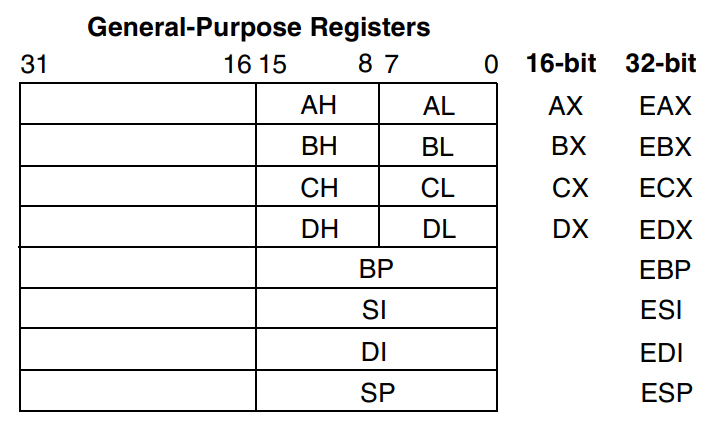
\includegraphics[width=10cm]{fig1.png}
\end{figure}

\h{Asembler:}
Program tłumaczący kod w języku asemblera na mod maszynowy.\\

\h{Język asemblera:}
W dużym uproszczeniu mnemoniczny zapis kodu maszynowego.\\

\h{Stos w x86:}
W Intelu x86 możemy potraktować część pamięci jako stos. Najczęściej jest on używany do przechowywania lokalnych argumentów funkcji oraz kodów powrotu. Warto odnotować, że adresy kolejnych elementów stosu nie wzrastają a maleją. Stos rośnie w x86 w dół.\\

\h{Typy danych w asemblerze:}
W asemblerze na architekturę x86 możemy wyróżnić typy danych:
\begin{itemize}
	\item \italic{Słowa kilkubajtowe} - bajt, słowo, słowo podwójne/poczwórne
	\item \italic{Liczby NB i U2} - wpierane bezpośrednio w sprzęcie
	\item \italic{Typy wskaźnikowe} - adresy  pamięci
	\item \italic{Pola bitowe} - pojedyncze bity zapisane w oddzielnych segmentach pamięci
	\item \italic{Łańcuchowe} - ciągi bajtów
	\item \italic{Wektorowe} - zbiory danych wspólnego typu (np. wektor liczb integer)
	\item \italic{Stałoprzecinkowe} - z lub bez znaku, BCD
	\item \italic{Zmiennoprzecinkowe} - standardu IEEE754
\end{itemize}

\end{document}